\documentclass[10pt]{article}

\usepackage{amssymb,amsmath,amsthm}
\usepackage{bm}
\usepackage{graphicx,subcaption}
\usepackage[letterpaper, top=1in, left=1in, right=1in, bottom=1in]{geometry}
\usepackage{siunitx}

\newtheorem{definition}{Definition}
\newtheorem{theorem}{Theorem}
\newtheorem{lemma}{Lemma}
\newtheorem{remark}{Remark}

\newcommand{\SO}{\ensuremath{\mathrm{SO}(3)}}
\newcommand{\tr}[1]{\ensuremath{\mathrm{tr}\left( #1 \right)}}
\newcommand{\abs}[1]{\ensuremath{\left| #1 \right|}}
\newcommand{\diff}[1]{\mathrm{d}#1}
\newcommand{\vect}[1]{\ensuremath{\mathrm{vec}\left[ #1 \right]}}

\newcommand{\liediff}{\mathfrak{d}}
\newcommand{\dft}{\mathcal{F}}
\newcommand{\real}{\ensuremath{\mathbb{R}}}
\newcommand{\sph}{\ensuremath{\mathbb{S}}}
\newcommand{\diag}{\ensuremath{\mathrm{diag}}}

\title{\vspace{-4ex}\textbf{Pendulum Collision\vspace{-4ex}}}
\date{}

\graphicspath{{Figs/}}

\begin{document}

\section{2D Pendulum}

\begin{figure}
	\centering
	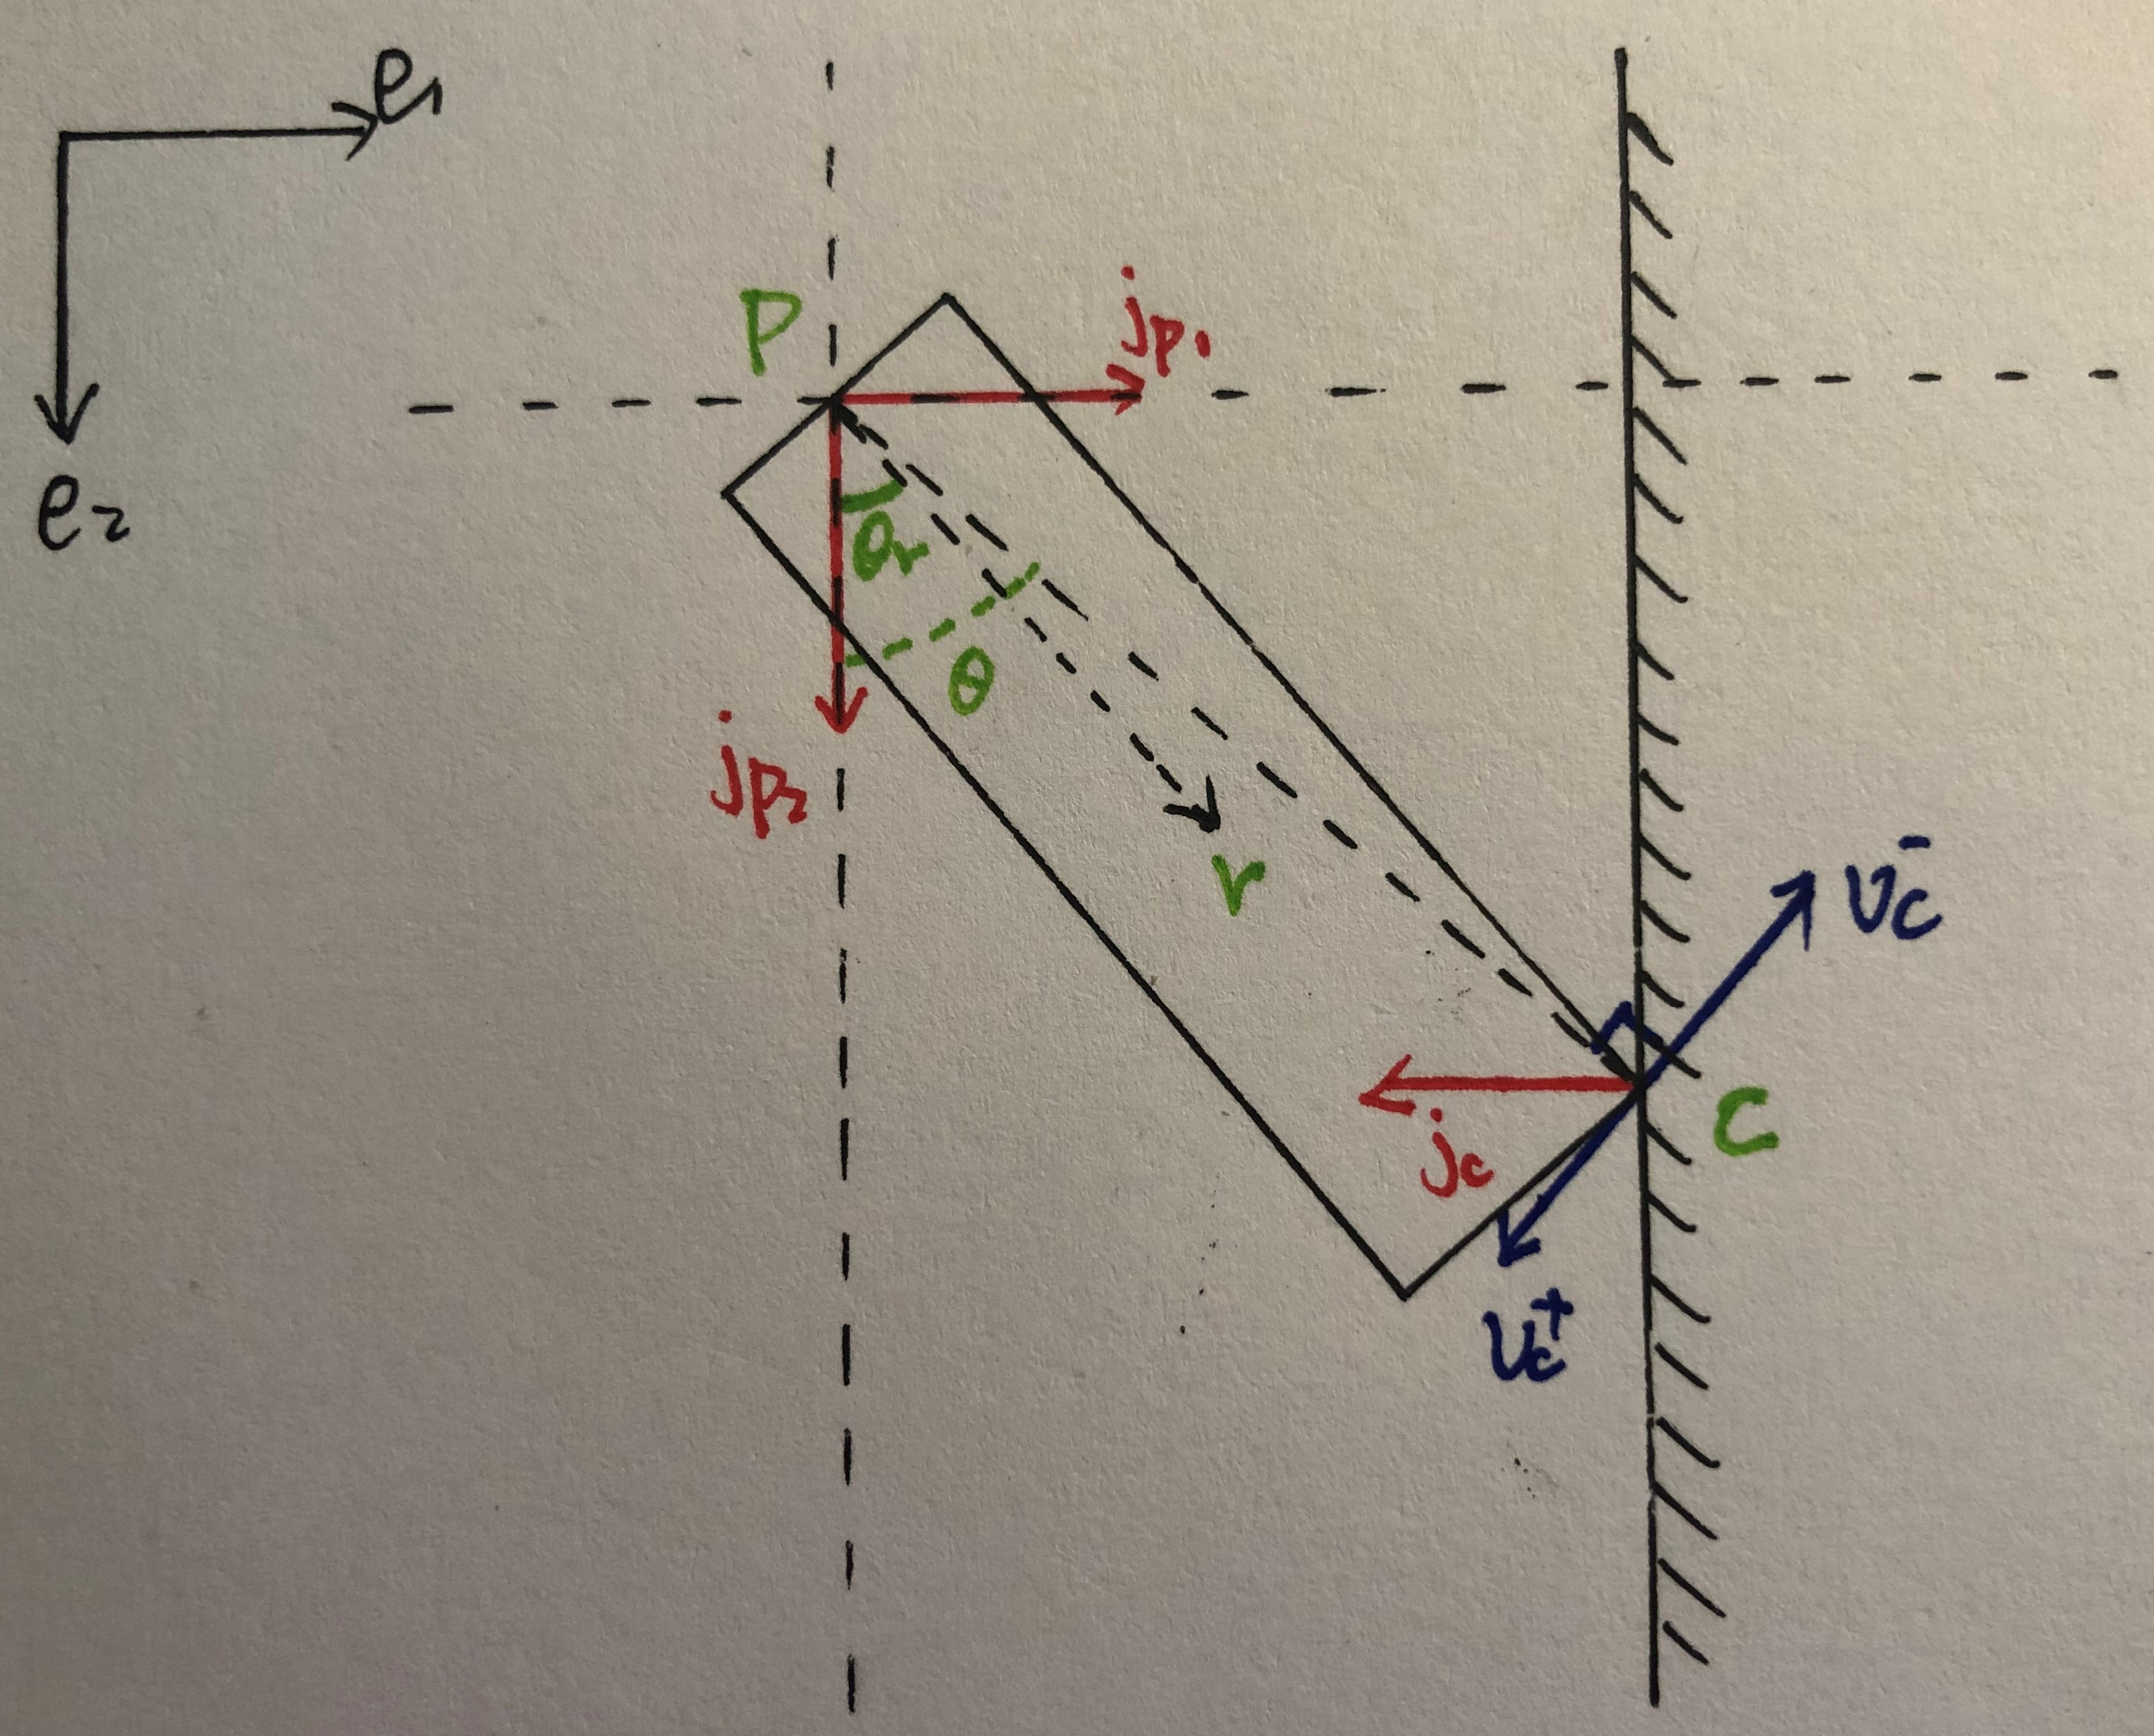
\includegraphics[scale=0.08]{collision_2D.JPG}
\end{figure}

Let $v_c^-$ and $v_c^+$ be the linear velocity of the pendulum at $C$ before and after collision.
Note that $v_c^-$ and $v_c^+$ must be perpendicular to $PC$ since the velocity at $C$ along $PC$ must be zero always.
For a frictionless collision, using the law of restitution, we have
\begin{align}
	v_c^+ \cdot e_1 = -\epsilon v_c^- \cdot e_1,
\end{align}
where $e_1$ is the normal direction of the wall, and $\epsilon\in[0,1]$ is the coefficient of restitution.
Since $v_c^-$ and $v_c^+$ are collinear, we have
\begin{align}
	|v_c^+|\cos\theta = \epsilon|v_c^-|\cos\theta \implies |v_c^+| = \epsilon|v_c^-|.
\end{align}
Let $\omega^-$ and $\omega^+$ be the angular velocity before and after the collision.
Then
\begin{align}
	\omega^- = \frac{\vec{PC}}{|PC|^2} \times v_c^-, \qquad \omega^+ = \frac{\vec{PC}}{|PC|^2} \times v_c^+ \implies \omega^+ = -\epsilon\omega^-.
\end{align}
Let $j_c$ be the magnitude of the collision impulse, and $j_{p_1}$, $j_{p_2}$ be the magnitude of the impulse at the hinge joint.
Then from linear momentum, we have
\begin{align}
	m(|\omega^+|+|\omega^-|)|r| \cos\theta_r &= j_c - j_{p_1}, \label{eqn:LM1-2d} \\
	m(|\omega^+|+|\omega^-|)|r| \sin\theta_r &= j_{p_2}.
\end{align}
From the angular momentum, we have
\begin{align}
	I(|\omega^+|+|\omega^-|) = j_c |PC| \cos\theta \label{eqn:AM-2d}.
\end{align}
The impulses $j_c$, $j_{p_1}$ and $j_{p_2}$ can be solved from \eqref{eqn:LM1-2d}-\eqref{eqn:AM-2d}.

\section{3D Pendulum}

\subsection{Collision Conditions}

\begin{figure}
	\centering
	\begin{subfigure}{0.49\textwidth}
		\includegraphics[scale=0.8]{collision_3D}
	\end{subfigure}
	\begin{subfigure}{0.49\textwidth}
		\includegraphics[scale=0.8]{collision_3D_annotate}
	\end{subfigure}
\end{figure}

The possible collision points form a circle $O$ on the wall.
Suppose the distance from the hinge joint to the wall is $d$, the height and radius of the pendulum is $h$ and $d$.
Then the radius of the circle is
\begin{align}
	r_{c} = \sqrt{r^2+h^2-d^2}.
\end{align}
The condition for collision is 
\begin{gather}
	\theta \geq \theta_0 \qquad \text{ i.e., } \qquad \arcsin(r_3 \cdot e_1) \geq \arcsin\frac{d}{\sqrt{h^2+r^2}} - \arcsin\frac{r}{\sqrt{h^2+r^2}} \\
	\omega \times \vec{PC} \cdot e_1 > 0, \label{eqn:col-cond-vel}
\end{gather}
where $\theta$ is the angle between the axial of the pendulum ($r_3$) and the $e_2$-$e_3$ plane.
Equation \eqref{eqn:col-cond-vel} guarantees the velocity at $C$ is into the wall.

\subsection{Collision Response}

Let $t$ be the tangent line of the circle $O$ at the collision point $C$.
Note that $t$ is in the blue plane which is perpendicular to $e_1$.
Then $t$ must also be the tangent line of circle $R$ at $C$, since otherwise the pendulum will penetrate through the wall.
Thus $t$ is perpendicular to the plane formed by $OC$ and $CR$.
Because $t$ is also perpendicular to $e_1$, $PO$, $OC$, $CR$ are on the same plane, and hence is $PR$.
Let the collision impulse be $-je_1$, then we have
\begin{align} \label{eqn:cr-am}
	\omega^+ - \omega^- = I^{-1}\left( \vec{PC} \times (-je_1) \right),
\end{align}
where $I = RJR^T$ is the inertia tensor in $e_{123}$ frame.
Also, from the law of restitution, we have
\begin{align} \label{eqn:cr-res}
	(\omega^+\times \vec{PC}) \cdot e_1 = -\epsilon (\omega^- \times \vec{PC}) \cdot e_1.
\end{align}
Equation \eqref{eqn:cr-am} and \eqref{eqn:cr-res} includes four independent equations, and have four unknown variables: $\omega^+$, $j$.
Thus $\omega^+$ can be solved.

Next, we try to simplify \eqref{eqn:cr-am} and \eqref{eqn:cr-res}.
Note that $\vec{PC} \times je_1$ is parallel to $t$, and thus to the plane of circle $R$.
If we assume $J = \diag(J_1,J_1,J_3)$, suppose $t = \begin{bmatrix} a & b & 0 \end{bmatrix}^T$ in the body-fixed frame used to calculate $J$.
Then it is clear $J^{-1} t = \frac{1}{J_1} t$, i.e., the change of angular velocity $\omega^+ - \omega^-$ is along $t$.
As a consequence, the linear velocity at $C$ along $t$ remains unchanged during the collision.
And the velocity change in the $OCR$ plane can be analyzed similarly as in the 2D case.
Thus, we have
\begin{align} \label{eqn:col_resp}
	\omega^+ = \omega^- - (1+\epsilon) (\omega^- \cdot t) t.
\end{align}
Note that the angular velocity along the axial axis is preserved during the collision.

\section{Uncertainty Propagation}

\subsection{Rate Function}
The rate function can be designed as a step function;
\begin{align}
	\lambda(R,\Omega) = \begin{cases}
		\lambda_{\text{max}}, &\text{if} \ \theta \geq \theta_0, \ R\Omega \times \vec{PC} \cdot e_1 \geq 0 \\
		0, &\text{else}
	\end{cases}.
\end{align}
The collision point $\vec{PC}$ can be calculated as
\begin{align}
	\vec{PC} = (h-r\tan\theta) r_3 + r\sec\theta e_1,
\end{align}
where $\theta$ is the angle between the axial axis and $e_2$-$e_3$ plane.
To make the transition smoother, the rate function can be modified as
\begin{align}
	\lambda(R,\Omega) = \begin{cases}
		\frac{\lambda_{\text{max}}}{2} \sin\left( \frac{pi}{2\theta_t}(\theta-\theta_0) \right) + \frac{\lambda_{\text{max}}}{2}, & \text{if} \ -\theta_t \leq \theta - \theta_0 \leq \theta_t, \ R\Omega \times \vec{PC} \cdot e_1 \geq 0 \\
		\lambda_{\text{max}}, & \text{if} \ \theta - \theta_0 > \theta_t, \ R\Omega \times \vec{PC} \cdot e_1 \geq 0 \\
		0, & \text{else}
	\end{cases}.
\end{align}

\subsection{Transition Kernel}

\subsubsection{No Noise}
Suppose there is no noise during the collision.
Then the transition kernel is given by
\begin{align}
	\kappa(R^-,\Omega^-,R^+,\Omega^+) = \delta_{\SO} \left( R^-(R^+)^T \right) \cdot \delta_{\real^2}(\Omega^+ - f(R^-,\Omega^-)),
\end{align}
where $\delta_{\SO}(R) = 0$ for all $R \neq I_{3\times 3} \in\SO$, and $\int_{R\in\SO} \delta_{\SO}(R) \diff{R} = 1$.
Similarly, $\delta_{\real^2}(x) = 0$ for all $x \neq 0 \in\real^2$, and $\int_{x\in\real^2} \delta_{\real^2}(x) \diff{x} = 1$.
Function $f$ is the same as the collision response \eqref{eqn:col_resp}:
\begin{align}
	f(R^-,\Omega^-) = (R^-)^T\left( \omega^- - (1+\epsilon)(\omega^- \cdot t^-) t^- \right),
\end{align}
where $\omega^- = R^-\Omega^-$, and $t^- = \frac{r_3^- \times e_1}{|r_3^- \times e_1|}$.

Then the integral can be simplified as
\begin{align} \label{eqn:int_simp1}
	&\int_{R\in\SO} \int_{x\in\real^2} \kappa(R^-,\Omega^-,R^+,\Omega^+) \lambda(R^-,\Omega^-) p_d(t,R^-,\Omega^-) \diff{\Omega^-} \diff{R^-} \nonumber \\
	= &\int_{x\in\real^2} \delta_{\real^2} (\Omega^+ - f(R^+,\Omega^-)) \lambda(R^+,\Omega^-) p_d(t,R^+,\Omega^-) \diff{\Omega^-}.
\end{align}
Note that
\begin{align} \label{eqn:delta_g}
	\delta_{\real^2} (\Omega^+ - f(R^+,\Omega^-)) = \delta_{\real^2} (\Omega^- - g(R^+,\Omega^+)).
\end{align}
The function $g$ is the inverse of $f$, given by
\begin{align}
	g(R^+,\Omega^+) = (R^+)^T \left( \omega^+ - \left( \frac{1+\epsilon}{\epsilon} \omega^+ \cdot t^+ \right) t^+ \right),
\end{align}
where $\omega^+ = R^+\Omega^+$, and $t^+ = \frac{r^+_3 \times e_1}{|r^+_3 \times e_1|}$.
Substitute \eqref{eqn:delta_g} into \eqref{eqn:int_simp1}, it can be further simplified as
\begin{align}
	&\int_{R\in\SO} \int_{x\in\real^2} \kappa(R^-,\Omega^-,R^+,\Omega^+) \lambda(R^-,\Omega^-) p_d(t,R^-,\Omega^-) \diff{\Omega^-} \diff{R^-} \nonumber \\
	= &\lambda(R^+,g(R^+,\Omega^+)) p_d(t,R^+,g(R^+,\Omega^+)).
\end{align}
Taking together, the discrete transition law is given by
\begin{align}
	\frac{\partial p_d(t,R,\Omega)}{\partial t} = \lambda(R,g(R,\Omega)) p_d(t,R,g(R,\Omega)) - \lambda(R,\Omega) p_d(t,R,\Omega).
\end{align}

\subsubsection{With Noise}
Suppose the angular velocity suffers a Gaussian noise during the collision
\begin{align}
	\Omega^+ = (R^-)^T\left( \omega^- - (1+\epsilon)(\omega^- \cdot t^-) t^- \right) + H_d\xi \triangleq \Omega^+_0 + \begin{bmatrix} H_d\xi \\ 0 \end{bmatrix},
\end{align}
where $H_d\in\real^{2\times 2}$, $\xi\in\real^2$ is standard normal, and the third row of $H_d$ is zero.
Let $G_d = H_dH_d^T$, and $\tilde{\Omega}$ be the first two elements of $\Omega$, then the transition kernel is given by
\begin{align} \label{eqn:kappa-noise}
	\kappa(R^-,\tilde{\Omega}^-,R^+,\tilde{\Omega}^+) = \delta_{\SO}(R^-(R^+)^T) \cdot \frac{1}{2\pi\sqrt{\det G_d}} \exp\left\{ -\tfrac{1}{2} \left(\tilde{\Omega}^+ - \tilde{\Omega}_0^+\right)^T G_d^{-1} \left(\tilde{\Omega}^+ - \tilde{\Omega}_0^+\right) \right\}.
\end{align}
Denote the second term on the right hand side of \eqref{eqn:kappa-noise} as $p_c(\tilde{\Omega}^+,R^-,\tilde{\Omega}^-)$, then the integral becomes
\begin{align}
	&\int_{R\in\SO} \int_{x\in\real^2} \kappa(R^-,\tilde{\Omega}^-,R^+,\tilde{\Omega}^+) \lambda(R^-,\tilde{\Omega}^-) p_d(t,R^-,\tilde{\Omega}^-) \diff{\tilde{\Omega}^-} \diff{R^-} \nonumber \\
	= &\int_{x\in\real^2} p_c(\tilde{\Omega}^+,R^+,\tilde{\Omega}^-) \lambda(R^+,\tilde{\Omega}^-) p_d(t,R^+,\tilde{\Omega}^-) \diff{\tilde{\Omega}^-} \\
	\approx & \sum_{i=1}^{Ng} p_c(\tilde{\Omega}^+,R^+,\tilde{\Omega}^-_i) \lambda(R^+,\tilde{\Omega}^-_i) p_d(t,R^+,\tilde{\Omega}^-_i) \Delta \tilde{\Omega}^-_i.
\end{align}
Thus, the discrete transition law is
\begin{align}
	\frac{\partial p_d(t,R,\tilde{\Omega})}{\partial t} \approx \sum_{i=1}^{Ng} p_c(\tilde{\Omega},R,\tilde{\Omega}^-_i) \lambda(R,\tilde{\Omega}^-_i) p_d(t,R,\tilde{\Omega}^-_i) \Delta \tilde{\Omega}^-_i - \lambda(R,\tilde{\Omega}) p_d(t,R,\tilde{\Omega}).
\end{align}

\end{document}

